%% das Papierformat zuerst
\documentclass[a4paper, 11pt]{article}
\usepackage[margin=3cm]{geometry}
\usepackage[utf8]{inputenc}
%\usepackage[T1]{fontenc}
\usepackage[fleqn]{amsmath} %left aligned equations
\usepackage{hyperref} % clickable refs
\usepackage{graphicx}
\usepackage[toc, numberedsection]{glossaries}
\usepackage{float}
\usepackage{amssymb}
\usepackage{calc}
\usepackage{enumitem} 
\usepackage{url}
\usepackage{parskip}
\usepackage{amssymb}
% http://tex.stackexchange.com/questions/17730/newcommand-and-spacing
\usepackage{xspace}
\usepackage{xparse}
% 'frame' option for figures
\usepackage[export]{adjustbox}
% fancy page headers
\usepackage{fancyhdr}
\usepackage{xcolor}
\usepackage{tabularx}
\usepackage{listings}
\usepackage{hyperref}
\usepackage{xstring}
\usepackage[lined,boxed,commentsnumbered]{algorithm2e}
\usepackage{makecell}
\usepackage{pifont}
\newcommand{\xmark}{\ding{55}}%
% page style
\pagestyle{fancy}
\fancyhead[R]{
\includegraphics[width=2cm]{../assets/kitlogo}}
\fancyhead[L]{\leftmark}
\fancypagestyle{plain}{
	\rhead{
\includegraphics[width=2cm]{../assets/kitlogo}}
	\lhead{\leftmark}
}

% TODO: template übersetzten

\makeglossaries

%Hack for referencing labels
\makeatletter
\def\namedlabel#1#2{\begingroup
    #2%
    \def\@currentlabel{#2}%
    \phantomsection\label{#1}\endgroup
}
\makeatother
% End: Hack for referencing labels

% Glossar: alle Einträge, aber ohne extra Referenzen
% http://tex.stackexchange.com/questions/115635/glossaries-suppress-pages-when-using-glsaddall
\newcommand*{\glsgobblenumber}[1]{}
\makeatletter
\newcommand*{\glsaddnp}[2][]{
  \glsdoifexists{#2}{
    \def\@glsnumberformat{glsgobblenumber}
    \edef\@gls@counter{\csname glo@#2@counter\endcsname}
    \setkeys{glossadd}{#1}
    \@gls@saveentrycounter
    \@do@wrglossary{#2}
  }
}
\renewcommand{\glsaddallunused}[1][]{
  \edef\@glo@type{\@glo@types}
  \setkeys{glossadd}{#1}
  \forallglsentries[\@glo@type]{\@glo@entry}{
    \ifglsused{\@glo@entry}{}{
      \glsaddnp[#1]{\@glo@entry}}}
}
\makeatother

\renewcommand{\glsnamefont}[1]{\mdseries #1} % glossary entries shouldn’t be bold

% Glossar

% So sieht ein Glossar-Eintrag aus:
%
%\newglossaryentry{dijkstra}{
%  name={Dijkstra’s Algorithmus},
%  description={ein Algorithmus, um den optimalen Pfad in einem gerichteten Graphen zu finden}
%}
%\newglossaryentry{arc}{
%  name={Arc-Flags},
%  description={eine Technik, um Routenberechnung zu beschleunigen},
%  see={dijkstra}
%}
%
% Und so kann er im Dokument verwendet werden:
%
% lorem ipsum dolor sit \gls{arc}, consectetur
%
% End: Glossar

% usage: \counteditem{prefix}{refName} -> item `/prefixXX/` with label `prefix:refName` (where XX is counted in increments of 10)
\makeatletter
\newcommand{\oitem}[2]{
  % define the counter
  \@ifundefined{c@oitem#1}{\newcounter{oitem#1}}{} % initialized at 0
  \addtocounter{oitem#1}{10}
  \item[\namedlabel{#1:#2}{/#1\arabic{oitem#1}/}]
}
\makeatother

% new page after section
\let\oldsection\section
\renewcommand\section{\clearpage\oldsection}

\newcommand{\mamidscreenshot}[1]{\includegraphics[width=\textwidth,frame]{#1}}

\newcommand{\uiel}[3]{\item \textbf{"#1" #2:} #3}

\definecolor{darkgreen}{rgb}{0.0, 0.5, 0.0}
\newcommand{\checkcomment}[1]{
	\def\temp{#1}
	\ifx\temp\empty
	\emph{}
	\else
	 \emph{Note: #1}
	\fi
}
\newcommand{\done}[1][]{{\color{darkgreen}\checkmark\checkcomment{#1}}}
\newcommand{\notdone}[1][]{{\color{red}\xmark\checkcomment{#1}}}


\begin{document}

\newcommand{\abbildung}[1]{\autoref{fig:#1}}
\newcommand{\mamid}{\textit{MAMID}\xspace}


%http://tex.stackexchange.com/questions/43002/how-to-preserve-the-same-parskip-in-minipage
\newlength{\currentparskip}
\newenvironment{minipageparskip}
{
        \setlength{\currentparskip}{\parskip}% save the value
	\begin{minipage}{\textwidth}% open the minipage
	\setlength{\parskip}{\currentparskip}% restore the value
} {
        \end{minipage}
}

\NewDocumentCommand{\refgo}{m}{%
  \IfHasLabel{#1}{%
    \sloppy\hyperref[#1]{\codeinline{\refgosymboltext{#1}}}%
  }{%
   \codeinline{#1}%
   %\colorbox{red}{\texttt{#1}}%
  }%
  \let\refdisplaytext\undefined%
}

%Refgo with alternative text
\NewDocumentCommand{\refgoalt}{m m}{%
	\IfHasLabel{#1}{%
		\sloppy\hyperref[#1]{\codeinline{#2}}%
	}{%
	\codeinline{#1}%
	%\colorbox{red}{\texttt{#1}}%
}%
\let\refdisplaytext\undefined%
}

% used to produce symbol names relative to the current scope
\NewDocumentCommand{\refgosymboltext}{m}{%
  % nibble the scope hierarchy: .gocurpackage.gocurtype.gocurmethod%
  \StrLen{\gocurpackage.}[\gocurlen]%
  \StrLeft{#1}{\gocurlen}[\refgosymbolCurComponent]%
  \IfStrEq{\refgosymbolCurComponent}{\gocurpackage.}{%
    % we are in scope of the package  %
      \StrGobbleLeft{#1}{\gocurlen}[\gocurremainingpath]%
      %
      \StrLen{\gocurtype.}[\gocurlen]%
      \StrLeft{\gocurremainingpath}{\gocurlen}[\refgosymbolCurComponent]%
      \IfStrEq{\refgosymbolCurComponent}{\gocurtype.}{%
        % we are in class scope       %
        \StrGobbleLeft{\gocurremainingpath}{\gocurlen}[\gocurremainingpath]%
        %
        \StrLen{\gocurmethod.}[\gocurlen]%
        \StrLeft{\gocurremainingpath}{\gocurlen}[\refgosymbolCurComponent]%
        \IfStrEq{\refgosymbolCurComponent}{\gocurmethod.}{%
          %
          \StrGobbleLeft{\gocurremainingpath}{\gocurlen}[\gocurremainingpath]%
          \gocurremainingpath%
        }{%
          \gocurremainingpath%
        }%
      }{%
        \gocurremainingpath%
      }%
  }{%
    % we are not in scope of the package%
    #1%
  }%
}

%%%%%%%%%%%%%%%%%%%%%%%%%%%%%%%%%%%%%%%%%%%%%%%%%%%%%%%%%%%%%%%%%%%%%%%%%%%%%%%%
%                       Util-commands that are dirty hacks
%                       to enable the helper commands

% evaluate #2 if the label #1 exists, else #3.
\makeatletter
\newcommand{\IfHasLabel}[3]{%
  \@ifundefined{r@#1}% declaring a label xyz defines r@xyz
               {#3}%
               {#2}%
}
\makeatother

% Styling of inline 'code', e.g. types.
\definecolor{codeinline-gray}{gray}{0.95}
\NewDocumentCommand{\codeinline}{m}{%
  % Specify inline code / command
  % Markdown equivalent: `#1`
  \colorbox{codeinline-gray}{\texttt{#1}}%
}

%%%%%%%%%%%%%%%%%%%%%%%%%%%%%%%%%%%%%%%%%%%%%%%%%%%%%%%%%%%%%%%%%%%%%%%%%%%%%%%%

%%%%%%%%%%%%%%%%%%%%%%%%%%%%%%%%%%%%%%%%%%%%%%%%%%%%%%%%%%%%%%%%%%%%%%%%%%%%%%%%
%                               Helper Commands
% ... defining types, methods, paramters, etc

% redefine \gocurpackage to the package name that the
%   subsequent \, \property, \method, etc belong too
\newcommand{\gocurpackage}{none}
\newcommand{\gocurtype}{}
\newcommand{\gocurmethod}{}

% an abstraction for declaring types, i.e. \struc or \interface
% #1: the type of type, i.e Struct or Interface
% #2: the name of the type
% #3: prologue
% #4: properties. list of \property
% #5: methods. list of \method
%
\NewDocumentCommand{\gotype}{m m +m +g +g +d<>}{%
  \subsection{#1 \codeinline{#2}}\label{\gocurpackage.#2}%
  % Make the current type name available in the scope of the class.
  % Useful for making labels.
  \renewcommand{\gocurtype}[0]{#2}% 
  #3%
  \IfValueT{#5}{%
    \subsubsection*{Fields}%
    \begin{description}%
      #5% list of \property
    \end{description}%
   }%
   \IfValueT{#4}{%
      \subsubsection*{Methods}%
      \begin{description}%
        %\setlength{\itemsep}{1em}
        #4%list of \method
      \end{description}%
   }%
   \IfValueT{#6}{%
      \subsection*{Enum Values}%
      \begin{description}%
          #6% list of \goenumitem
      \end{description}%
   }%
   \renewcommand\gocurtype[0]{}%
}
\NewDocumentCommand{\jsview}{m +m}{\gotype{View}{#1View}{#2}}
\NewDocumentCommand{\jscontroller}{m +m}{\gotype{Controller}{#1Controller}{#2}}
\NewDocumentCommand{\struct}{m +m +g +g}{\gotype{Struct}{#1}{#2}{#4}{#3}}
\NewDocumentCommand{\interface}{m +m +g}{\gotype{Interface}{#1}{#2}{#3}}
\NewDocumentCommand{\goenum}{m +m +m}{\gotype{Enum}{#1}{#2}<#3>}
\NewDocumentCommand{\typealias}{m r[] +g}{%
  \subsection{Type Alias \codeinline{#1 $\equiv$ #2}}\label{\gocurpackage.#1}%
  #3
}

\NewDocumentCommand{\beginpackage}{m}{
	\renewcommand{\gocurpackage}{#1}\label{\gocurpackage}
}

\NewDocumentCommand{\reftype}{m}{\refgo{\gocurpackage.#1}}

% \property is used to declare fields of a struct
\NewDocumentCommand{\property}{m o +g}{
  \item[\codeinline{#1\hspace{0.1cm}:\hspace{0.1cm}#2}]\label{\gocurpackage.\gocurtype.#1}\hfill %(line break for the poor)
  \IfValueT{#3}{%
    \par
    #3
  }%
}
\NewDocumentCommand{\refproperty}{m}{\refgo{\gocurpackage.\gocurtype.#1}}

\NewDocumentCommand{\goenumitem}{m +m}{
  \item [\codeinline{#1}]\label{\gocurpackage.\gocurtype.#1} #2
}

% \method is used to declare a struct's method set.
\NewDocumentCommand{\method}{m o d() +m}{
\renewcommand\gocurmethod[0]{#1}%
\item[\codeinline{#1(\IfValueT{#3}{$\cdot$})\IfValueT{#2}{\hspace{0.1cm}:\hspace{0.1cm}#2}}]\label{\gocurpackage.\gocurtype.#1}\hfill %(line break for the poor)
  \IfValueT{#3}{
    \begin{description}
      #3 % should only contain \param
    \end{description}
  }
  \par
  #4
  \renewcommand\gocurmethod[0]{}%
}
\NewDocumentCommand{\refmethod}{m}{
	\refgo{\gocurpackage.\gocurtype.#1}
}

% \param is used to declare paramters of a \method -> check \method for details
\NewDocumentCommand{\param}{m o +m}{%
  \item[\codeinline{#1\hspace{0.1cm}:\hspace{0.1cm}#2}]\label{\gocurpackage.\gocurtype.\gocurmethod.#1} #3
}

\NewDocumentCommand{\refparam}{m}{
  \refgo{\gocurpackage.\gocurtype.\gocurmethod.#1}
}


%%%%%%%%%%%%%%%%%%%%%%%%%%%%%%%%%%%%%%%%%%%%%%%%%%%%%%%%%%%%%%%%%%%%%%%%%%%%%%%%

%%%%%%%%%%%%%%%%%%%%%%%%%%%%%%%%%%%%%%%%%%%%%%%%%%%%%%%%%%%%%%%%%%%%%%%%%%%%%%%%

%%%%%%%%%%%%%%%%%%%%%%%%%%%%%%%%%%%%%%%%%%%%%%%%%%%%%%%%%%%%%%%%%%%%%%%%%%%%%%%%

% alle Glossareintraege
\newacronym{gui}{GUI}{Graphical User Interface}
\newacronym{cli}{CLI}{Command Line Interface}
\newacronym{CRUD}{CRUD}{Create / Read / (Update|Modify) / Delete}
\newacronym{ICMP}{ICMP}{Internet Control Message Protocol}
\newacronym{API}{API}{Application Programming Interface}
\newacronym{JSON}{JSON}{JavaScript Object Notation}
\newacronym{HTTP}{HTTP}{HyperText Transfer Protocol}
\newacronym{LAN}{LAN}{Local Area Network}
\newacronym{WAN}{WAN}{Wide Area Network}

\newglossaryentry{cluster}{
	name={cluster},
	description={Aggregation of \glspl{host}},
	plural={clusters}
}
\newglossaryentry{MongoDB}{
	name={MongoDB},
	description={A NoSQL based database server},
	plural={MongoDB}
}
\newglossaryentry{replica set}{
	name={replica set},
	description={Multiple \gls{MongoDB} instances distributed over multiple \glspl{host} sharing a copy of the same data},
	plural={replica sets}
}
\newglossaryentry{sharding}{
	name={Sharding},
	description={A type of \gls{MongoDB} deployment where data sets are spread across multiple \glspl{host} or \glspl{replica set}. \\ More information: {\small \url{https://docs.mongodb.com/manual/sharding/}}}
}
\newglossaryentry{administrator}{
	name={administrator},
	description={The person responsible for managing the hardware \& software deployed on the \gls{cluster}. Uses \mamid for \gls{MongoDB} \gls{replica set} administration},
	plural={administrators}
}
\newglossaryentry{host}{
	name={host},
	description={Network node with a unique hostname},
	plural={hosts}
}
\newglossaryentry{slave}{
	name={slave},
	description={Program running on \gls{host} managing \gls{MongoDB} processes},
	plural={slaves}
}
\newglossaryentry{master}{
	name={master},
	description={Program responsible for managing \glspl{slave} and providing \acrshort{API} for \gls{cluster} management},
	plural={masters}
}
\newglossaryentry{inventory}{
	name={inventory},
	description={Persistently stored list of slaves and their state (see \ref{D:Inventory})},
	plural={inventories}
}
\newglossaryentry{active mode}{
	name={active mode},
	description={Marks the \gls{slave} as available to host \gls{MongoDB} processes that are be part of \glspl{replica set}.},
	plural={active modes}
}
\newglossaryentry{maintenance mode}{
	name={maintenance mode},
	description={Marks the \gls{slave} as unavailable \& inhibits reconfiguration through \gls{master}, but does not otherwise affect running \gls{MongoDB} instances on the \gls{host}.},
	plural={maintenance modes}
}
\newglossaryentry{disabled mode}{
	name={disabled mode},
	description={A \gls{slave} in this mode does not run any \gls{MongoDB} instances controlled by the \gls{master}, hence has no \gls{MongoDB} instances in any \gls{replica set}.},
	plural={disabled modes}
}
\newglossaryentry{risk group}{
	name={risk group},
	description={A set of \glspl{host} sharing a common risk of failure, e.g. a shared power supply. Modeled through sets of \glspl{slave} since a 1:1 relationship exists between hosts and slaves},
	plural={risk groups}
}
\newglossaryentry{persistent storage}{
	name={persistent storage},
	description={Storage capable of storing data between power outage},
	plural={persistent storages}
}
\newglossaryentry{volatile storage}{
	name={volatile storage},
	description={Storage incapable of storing data between process lifetime},
	plural={volatile storages}
}
\newglossaryentry{root data directory}{
	name={root data directory},
	description={Base directory holding all files of a \gls{slave} and its \gls{MongoDB} instances},
	plural={root data directories}
}
\newglossaryentry{arbiter}{
	name={arbiter},
	description={In charge of breaking ties on a \gls{replica set} election with even number of members. More information: {\small \url{https://docs.mongodb.com/manual/core/replica-set-elections/}}},
	plural={arbiters}
}
\newglossaryentry{degraded}{
	name={degraded},
	description={State of a \gls{replica set} with member in \gls{maintenance mode} or \gls{disabled mode} or otherwise reporting failure},
	plural={degraded}
}

\begin{titlepage}
\makeatletter
\begin{center}
~\\[4em]
{\Huge MAMID}\\[.8em]\huge{Monitor and Manager for In-memory Databases}\\[2em]
{\huge Implementation \& Testing}\\[1em]
{\large\today}\\[2.5em]
{\LARGE
Niklas Fuhrberg\\
Anton Schirg\\
Christian Schwarz\\
Janis Streib\\
Bob Weinand\\[3em]}
{\Large supervised by}\\[2em]
{\LARGE
Dr Marek Szuba\\[1em]}
{\Large at}\\[1em]
{\LARGE
Karlsruhe Institute of Technology\\
SCC\\[2em]}
{\color{gray}
  \small Document Version: \newtheorem{theorem}{Theorem}


\section{master}

\renewcommand{\gocurpackage}{model}
\renewcommand{\gocurpackage}{master}

\struct{ClusterAllocator}{
  The \refstruct{ClusterAllocator} determines the layout of the cluster managed by \mamid.

  It attempts to fulfill the constraints defined through the model objects, in particular
  \begin{itemize}
    \item A \refgo{model.ReplicaSet}'s \refgo{VolatileNodeCount} \& \refgo{PersistentNodeCount}
    \item The \refgo{model.Slave}'s allowed number of Mongod instances
          (\refgo{MongodPortRangeBegin} to \refgo{MongodPortRangeEnd}).
    \item The \refgo{model.Slave.SlaveState}
    \item The configured \refgo{model.RiskGroup}s.
  \end{itemize}

  An iterative algorithm is employed to decide on a cluster layout described through
  \refgo{model.Mongod.DesiredState}s that
  \begin{itemize}
    \item attempts to fulfill the above constraints
    \item attempts an even distribution of Mongods on the different cluster hosts
    \item is a minimal change in comparison to the previous layout
  \end{itemize}

  \begin{theorem}{Idempotence of the ClusterAllocator}
    \label{theorem:idempotence_clusterallocator}
    Let $l$ be a layout of the cluster. Then $ClusterAllocator(ClusterAllocator(l)) = ClusterAllocator(l)$.
  \end{theorem}

}{
  \property{DB}[gorm.DB]{Initialized handle to the database.}
  \property{BusChannel}[chan interface{}]{Initialized channel to the application bus.} %TODO ref}
}{
  \method{LayoutCluster}{Lay out the cluster as described above.}
}

\subsubsection{Pseudocode}

The \refstruct{master.ClusterAllocator} is crucial to the stable operation of the \mamid-managed cluster.\\
Hence, it is worth defining the implementation of \refgo{master.ClusterAllocator.LayoutCluster} through pseudocode. %TODO parentheses

While studying the algorithms below, the reader should keep in mind that
\begin{itemize}
  \item changes in the cluster layout $\equiv$ change or creation of \refgo{model.Mongod.DesiredState} 
  \item the \refgo{model.Mongod.ObservedState} may change after an arbitrary amount or even never.\\
  \item changes to a ReplicaSet must not violate or further worsen the high-availibility constraints,
        in particular \refgo{model.ReplicaSet}'s \refgo{VolatileNodeCount} \& \refgo{PersistentNodeCount}\\
        $\implies$ Mongods in \refgo{model.MongodExecutionState.Recovering} are an important special-case.
\end{itemize}

\newcommand{\pluseq}{\mathrel{{+}{=}}}
\newcommand{\minuseq}{\mathrel{{-}{=}}}
\SetKwInOut{Input}{input}
\SetKwInOut{Output}{output}
\SetKwProg{Fn}{Function}{}{}
\SetKw{Invariant}{invariant}
\IncMargin{0.5em}

Invariant: Algorithm(Algorithm(x)) = Algorithm(x)

Otherwise oscillations could occur

Most interesting case: Set a slave to disabled. Then a new Mongod should be spawned and recover and when it is done the old disabled one can be deleted.

\begin{algorithm}

\caption{Count members of a Replica Set that are \& intended to be in stable state (running)}

\Input{ReplicaSet $r$}
\Output{Number of $p_e$ and $v_e$ member processes of $r$ that are fully operational and are planned to remain in that state.}
\BlankLine
\Fn{EffectiveMemberCount(r ReplicaSet)}{

$p_e, v_e = 0$

\For{$m \in \text{r.Mongods}$}{
	\If{$\text{m.ObservedState.ExecutionState} = Running$ \\ 	%	#this line evaluates to false if m.ObservedState = NULL
		$\land \text{m.DesiredState.ExecutionState} = Running$}{ %#this line evaluates to false if m.DesiredState = NULL 

		\uIf{$m.ParentSlave.PersistentStorage$}{
			$p_e \pluseq 1 $
		}\Else{
			$v_e \pluseq 1 $
		}
	}
}
\Return $p_e, v_e$
}
\end{algorithm}


\begin{algorithm}
\caption{Destroy members of disabled replica sets where possible without violating p/v constraints.}
\ForEach{r in ReplicaSets}{
	
	$p_e, v_e \gets $ EffectiveRunningMembers(r)
	
	\ForEach(// same for persistent and volatile){$\textbf{x}_e \in \{p_e, v_e\}$}{
		\While{$x_e > r.\textbf{x}$}{
			\textbf{destroy} any $m \in r.Mongods$ where $m.ParentSlave$ is $\textbf{x} \land \textbf{disabled}$\;
			$\textbf{x}_e \minuseq 1$
		}
		
		\Invariant minimum number of disabled slaves are running members of $r$\;
		
		\While{$\textbf{x}_e > r.\textbf{x}$}{
			\textbf{destroy} any $m \in r.Mongods$ where $m.ParentSlave$ is $\textbf{x}$\;
			$\textbf{x}_e \minuseq 1$
		}
		
		\Invariant at most $r.\textbf{x}$ members 
	}
	
	\Invariant \textit{desired state}: at most (r.p|r.v) member processes of $r$\;
	// desired state = the state that will be deployed
	
}
\end{algorithm}

\begin{algorithm}
\caption{Count recovering and active members of a Replica Set}

\Input{ReplicaSet $r$}
\Output{Number of $p_a$ and $v_a$ member processes of $r$ that \begin{itemize}
		\item are \textbf{recovering}, i.e. soon-to-be fully operational
		\item fully operational (\textbf{running})
	\end{itemize} and should actually be in that state.}
\BlankLine
\Fn{AlreadyAddedMemberCount(r ReplicaSet)}{
	$p_a, v_a = 0$
	
	\For{$m \in \text{r.Mongods}$}{
		\If{$\text{m.ParentSlave.ConfiguredState} != Disabled$ \\
			$\land \text{m.DesiredState.ExecutionState} != NotRunning$}{ 
			
			\uIf{$m.ParentSlave.PersistentStorage$}{
				$p_a \pluseq 1 $
			}\Else{
			$v_a \pluseq 1 $
		}
	}
}
\Return $p_a, v_a$
}
\end{algorithm}

\begin{algorithm}
\caption{Spawn Mongods on under-provisioned Replica Sets respecting RiskGroup \& p/v constraints.}

$p_a, v_a \gets $ AlreadyAddedMemberCount(r)

\ForEach(// same for persistent and volatile){$\textbf{x}_a \in \{p_a, v_a\}$}{

	%# TODO need to fill the queue. only ReplicaSets which 'need' (use p_* to define what need means) are in  the queue 
	$RQ \gets$ PriorityQueue(R)\;% "relative amount of missing members")\;
	$RGSQ \gets$ map[RiskGroup]PriorityQueue(Slaves of RiskGroup)\;%, "relative amount of available Mongod ports")\;
	
	\While{$r = RQ.pop()$; $r \neq nil$}{
	
		\Invariant $r$ needs a member of type $\textbf{x}$
		
		// find $x$-slave $s$ in a risk group $g$ with no other Mongod of $r$ in $g$\;
		$candidates \gets \{g \mid g \in RGSQ.keys \land \text{r has no member in g}\}$\;
		$g \gets$ ARGMAX($g \in candidates$, RGSQ[g].PeekPriority())\;
		\uIf{$g \neq nil$}{
			$s \gets RGSQ[g].pop()$\;
			\Invariant $s$ has at least one free port\;
			spawn new Mongod $m$ on $s$ and add it to $r.Mongods$\;
			compute $MongodState$ for $m$ and set the $DesiredState$ variable\;
			
			\If{$r$ needs another member of type $\textbf{x}$}{
				$RQ.insert(r)$ // recompute priority
			}
			
			\If{$s$ has free ports}{
				$RGSQ[g].insert(s)$ // recompute priority
			}
			
			
		} \Else{
			yield error\;
			continue\;
		}
		
	
	}

}

\end{algorithm}


}
\end{center}
\makeatother
\end{titlepage}
\newpage
\tableofcontents
\newpage

\section{Introduction}

This document describes the design of the Application \mamid (\emph{Monitor and Manager for In-memory Databases}).

It thorougly explains the architecture of a \mamid deployment, the distribution of responsibilites among the various components,
individual Go structures, their methods and the relationships among them.

While the textual documentation delivers detailed information on individual components, the various UML diagrams
--- and in particular the class diagram --- clarify the interoperation between components and the architecture of \mamid.

In order to facilitate lecture of this document, the reader should be familiar with the contents of the \emph{Functional Specification}
document.\\
In particular, the following sections of the \emph{Functional Specification} are crucial for proper understanding of the
application design:
\begin{itemize}
  \item the technical terms introduced listed in the \emph{Glossary}
  \item the naming of \mamid components as described in the \emph{System Model}.
\end{itemize}

\subsection{Note: UML and Go}

The authors found it difficult to apply certain concepts of the \emph{Unified Modeling Language} to a Go application design.

The following conventions were employed during the design phase:

\begin{itemize}
        \item UML \codeinline{<<enum>>} does not exist in Go. However, it can be simulated using package constants with the \codeinline{<<enum>>} type as \textbf{shared unique prefix}. 

                \textbf{Example}: \codeinline{EnumType.Item1} maps to \codeinline{EnumTypeItem1} in the Go implementation.
        %TODO more?
\end{itemize}

The reader should further recognize the remarks on the UML modeling of the \refgo{gui} in section \ref{gui:beginsection}.

\section{Deviation from the Functional Specification}

The design phase revealed flaws in the \emph{Functional Specification} that have been addressed as follows.

\subsection{Root Data Directory (MC80, F40, Section 9.3.1)}

The \emph{Root Data Directory} is no longer specified in the master's inventory using the GUI.\\
Instead, it is passed directly to the slave via a command line flag parsed by the slave executable.

Changing the value on a slave with \refgo{msp.MongodState.Running} \codeinline{Mongods} results in a situation where either
all Mongds on the slave need to be temporarily destroyed or a special-case transition needs to be implemented.
Neither alternative is desirable.

Furthermore, changing the value is usually related to manual administrative action on the specific slave host.\\
Hence, moving the parameter to the command line flags of the slave simplifies both implementation and administrative work.

\subsection{Slave Mode \emph{unknown} \& Slave Error Handling (Section 5.3.1)}

The \emph{Functional Specification} declares four slave modes: \emph{active, maintenance, disabled, unknown}.\\
The \emph{unknown} mode would be presented to the user in case of
\begin{itemize}
  \item state mismatch
  \item monitoring errors
  \item communication errors
  \item deployment errors
\end{itemize}

The error handling architecture described in this document is more transparent and allows for actual debugging of an error.

Hence, the \emph{unknown} state is replaced by more fine grained error reporting.
Since it was a state only set by the master, this change has fairly low impact on other parts of the design.

\subsection{Other Optional Criteria}

The application architecture presented in this document is designed with extensibility in mind.\\
The authors are confident that a majority of the optional criteria listed in the \emph{Functional Specification} can be implemented
transparently, i.e. without greater changes to the existing architecture.

However, the authors consider the implementation of optional criteria mostly a question of time constraints during the
implementation phase, not one of general feasibility.

\section{Overview}

\mamid is a manager for database clusters, facilitating creation, administration and monitoring of a MongoDB Replica Set deployment.

Explicit support for volatile storage on primary Replica Set members with lower-prioritized secondaries on persistent
storage is a key differentiator of \mamid.

As the manager of such distributed systems with high-availibility requirements, \mamid faces a series of non-trivial problems:
\begin{itemize}
  \item unreliable hardware
  \item unreliable communication between nodes
  \item resilience against unexpected failures of the above 
  \item finding a deployment layout that fulfills a set of availibility requirements
  \item monitoring \& state tracking of the deployed MongoDB processes
  \item abstraction of the above complexity from the administrator
  %TODO more?
\end{itemize}

In order to achieve these goals, a distributed architecture is necessary.

\mamid implements several well-established design patterns, facilitating understanding of design and implementation and improving
testability of individual components.

As specified in the \emph{Functional Specification}, the language of choice for all components but the GUI is \emph{Golang}.
While \emph{Golang} can be considered a object-oriented language, it differs from languages like \emph{Java} in certain critical approaches:
\begin{itemize}
  \item no generics
  \item no classes, only \codeinline{struct} with \emph{method sets}
  \item this is most notable in the lack of \emph{Constructors} and \emph{inheritance}
  \item however, inhertance can be simulated to a certain degree through \emph{embedding} %TODO ref go spec
\end{itemize}

Overall, this leads to a situation where many traditional design patterns do not apply as well (as e.g. to Java) and hence need
to be adopted.

Given these constraints, \mamid still employs a variety of design patterns across its different components:

% GUI Design pattersn
The architecture of the \refgo{gui} follows the \textbf{Model-View-Controller} pattern.
% is this actually MVC? @janis should elaborate on this.
% TODO explain in short the idea of MVC proposed by Angular. It should be written down somewhere -> quote it

% Master Design Patterns
The \textbf{Client/server architecture pattern} is used to decouple the \refgo{gui} functionality from the \refgo{master}:
The \refgo{gui} acts as a frontend to the functionality provided by the \refgo{master} HTTP API (\refgo{masterapi}).

Being the most complex package of the project, several decoupling patterns are employed in the \refgo{master}:

The \textbf{repository pattern} is the most one employed inside the \refgo{master}:
The external \refgo{gorm} database abstraction layer holds several tables of the structures in \refgo{model}.\\
\refgoalt{master.Monitor}{Monitor},  \refgoalt{master.ProblemManager}{ProblemManager},
\refgoalt{master.Deployer}{Deployer} and  \refgoalt{master.ClusterAllocator}{ClusterAllocator} are loosely coupled and communicate mostly by
modifying the database.\\
Furthermore, a variation of the \textbf{publish/subsribe pattern} is implemented by the \refgo{master.Bus}.

% MasterSlave Protocol
The \textbf{remote proxy} decoupling pattern is employed in the {Master Slave Protocol (\refgo{msp}) package:
it implements communication bewteen \refgo{master} and \refgo{slave}.
\refgo{msp.MSPClient} exposes RPC stubs that call the the \refgo{msp.MSPConsumer} implemented on the \refgo{slave}.
Another term used to describe this relationship between master and slaves is the \textbf{Multi-Server/Single-Client architecture}.
%TODO or is it peer2peer? check SWT slides

% Slave design patterns
\textbf{Dependency injection} is employed extensively in both \refgo{master} and \refgo{slave} to increase testability through mocks.
A good example for this are the references to \codeinline{gorm.DB} passed into \refgoalt{master.Monitor}{Monitor},  \refgoalt{master.ProblemManager}{ProblemManager},
 \refgoalt{master.Deployer}{Deployer} and  \refgoalt{master.ClusterAllocator}{ClusterAllocator}.

% Notification Manager patterns
The \textbf{strategy pattern} is used inside the \refgo{notifier} to encapsulate the concrete notification delivery
to per communication channel (\refgo{notifier.Notifier}, increasing extensibility for different communication channels in the future.
% TODO actually a strategy or more of a template method?

%TODO more design patterns

\section{Design Improvements}

In accordance with the project supervisor, a text-based delta between the original and implemented application design
is beyond the scope of this document.

However, to facilitate understanding and future maintenance of the code base, the design document has been updated to the state of
the implementation at the time of writing this document.

The purpose of this section is to provide an overview of the reasoning behind the design changes.

% one subsection per problem encountered during implementation

\subsection{Master: Database-Related Changes}

During the design phase of the project, it was decided to use the \refgo{gorm} ORM layer and a relational database as the backing store
for \mamid application data.

While never officially stated, the developers assumed SQlite 3 to be sufficient for the purposes of \mamid.

This assumption was proven wrong when enough of the master modules were implemented to reveal the limited capabilities of SQlite 3 regarding
concurrent access: updating a single row or column in the database effectively requires an exclusive lock on the entire database (see https://www.sqlite.org/lockingv3.html).
The various master components however udpate (disjoint!) rows or columns in parallel.

Given a substantial part of the master codebase had already been written expecting this behavior, the developers decided to switch to
PostgreSQL, a well-established open source relational database (see https://www.postgresql.org/).

PostgreSQL
\begin{itemize}
\item compiles in its most recent version 9.5.4 on the primary target operating system \textit{OpenIndiana 151a9} (also with TLS support)
\item allows for the degree of parallel database access required by the master
\item has features like foreign keys, data type checking and referential actions enabled by default %TODO ref
\item allows for redundant deployments \& zero downtime backups through the \codeinline{pg\_dump(1)} utility (optional criteria) %TODO ref
\item thus significantly reduces the risk of a corrupted database.
\end{itemize}

However, switching to PostgreSQL revealed flaws in the database schema auto-generated by the \refgo{gorm} ORM layer:

\begin{itemize}
\item Foreign keys and referential actions need to be defined as Go Field Tags in the model definition.
\item Schema migrations are only half-heartedly supported.
\end{itemize}

It was decided to define the database schema in plain SQL and to implement support for creating and migrating the schema in \mamid. %TODO this ok?

Effortless compatibility to \refgo{gorm} is maintained by following the documented conventions for naming columns (see http://jinzhu.me/gorm/models.html\#conventions) .

\subsection{Master: Cluster Allocator Prioritization Datastructures}

The \refgo{master.ClusterAllocator} is crucial for the stable operation of the \mamid-managed cluster.

The design document contains a pseudocode implementation of the \refgo{master.ClusterAllocator} algorithms managing Replica Set members.

However, pseudocode usually does not map directly to the concrete implementation.

For the implementation of MAMID, the priority queue datastructures used in the Cluster Allocator pseudocode proved impractical to implement:

\begin{itemize}
\item The master architecture follows the \textit{repository pattern}, meaning that decoupled components work together by sharing data
through the central database.
\item The Cluster Allocator algorithms need read access to a a substantial amount of the cluster model stored in the database
      in order to make allocation decisions.
\item The \refgo{gorm} ORM layer cannot record fine-grained changes to objects (missing dynamism in Go).
      Hence, saving updates to an object graph to database leads to an update of all attributes,
      inducing conflicting transactions with other components of MAMID.
\item Keeping the priority queue datastructures in sync with the database state during a \refgo{master.ClusterAllocator} run
      appears to be impossible with \refgo{gorm}.
\end{itemize}

Given these problems, the priority queues where replaced by SQL queries encoding the prioritization criteria.
Several SQL views were introduced to keep the prioritization queries concise and improve performance.
Testing did not reveal performance problems with the \refgo{master.ClusterAllocator} implementation.

\subsection{Replica Set Deployment with Keyfiles}\label{:di:keyfiles}

MongoDB supports several mechanisms for internal authentication between members of a Replica Set. The only mechanism available on the
the target operating system \textit{OpenIndiana 151a9} is authentication through a shared secret (\textit{keyfile}).

The supervisor's desire to have the deployed Mongods authenticate themselves to each other using this meachanism was not mentioned 
until 1.5 weeks before the implementation deadline. %TODO validate

Implementation of the feature proved problematic: Mongod instances started with the \textit{keyfile} parameter disable the \textit{localhost exception}
as soon as a Replica Set is configured and activate \textit{user access control}. %TODO review and ref
This was incompatible with the assumption made during the design phase that a Mongod would be always configurable by a its system user without authentication.

Hence, support for keyfiles required substantial changes to the deployment process late in the implementation phase:

\begin{itemize}
  \item Represent keyfile data in the Model \& MSP
  \item Represent user credential data in the Model \& MSP
  \item Support deployment of keyfiles in Master \& Slave
  \item Support authentication in the \refgo{slave.MongodConfigurator} by defining a \textit{management user}
  \item Deal with various edge-cases related to MongoDB \textit{write-concern} and the \textit{sharding role} of a Mongod
  \item Allow the user to retrieve keyfile and \textit{management user} credential through the GUI,
        e.g. to create additional users or configure sharding configuration servers.
\end{itemize}

Adapting the deployment process to work with the \textit{localhost exception} proved time-consuming.

In order to meet the implementation deadline, the \textit{keyfile} and \textit{management user} are currently

\begin{itemize}
  \item generated using a PRNG on first launch of the master
  \item global to all Mongods in the cluster
  \item unchangeable through the GUI / API.
\end{itemize}

The developers are aware of the security problems this situation implies and furthermore recommend using a target platform that supports
the MongoDB x509 authentication mechanism. %TODO ok?

\subsection{Slave: Mongod \& Replica Set Configuration}

The various edge-cases and subtleties of MongoDB were underestimated during the design phase of \mamid.

In particular, the following problems complicated and delayed the slave implementation:
\begin{description}
\item[Replica Set Initiation] Initiation must happen from a single Mongod in the soon-to-be Replica Set.
     This prohibits the original idea of simply broadcasting a state description to all Slaves hosting Mongods of the Replica Set,
        as is done once the ReplicaSet is initiated.
     A separate MSP protocol message \refgo{msp.RsInitiateMessage} was introduced and other sub-datastructures refactored, allowing
        a coordinated initiation of the Replica Set.
\item[User Access Control] The introduction of \textit{user access control} complicates the retrieval of Mongod state since most MongoDB
        commands relevant to the \refgo{master.Monitor} are only allowed when authenticated.
        The slave needs to cache the \textit{management user} credential received through the MSP.
\item[Situations without Primary] A Replica Set with a majority of Mongods unreachable cannot elect a new Primary.
        However, reconfiguring the Replica Set without overriding safety checks (\codeinline{force=true}) is not possible then.
        \mamid itself should not make the decision to override the safety checks because this behavior could lead to data loss.
\end{description}

Making the slave compatible with the the problems described above led significant bloat in the \refgo{slave.MongodConfigurator}.

To increase maintainability, the interaction with the MongoDB API was extracted into a private MongoDB API wrapper (\refgo{slave.mgoContext}).

\subsection{We realized: administrator needs more details on the deployment of the cluster in order to use it for applications}

=> GUI needs to display more information
    - Mongods of Replica Sets
    => requirement for Mongod API endpoint (expose what is already in the Master database)

=> Useful gimmics for the admin: ready to copy-to-clipboard 
    - command lines for starting a sharding config server
    - MongoDB URL useful for pasting into application configuration running on top of a Replica Set

\subsection{Original GUI draft does not scale well to 80-100 machines }

- use dense UI elements
- implement filtering functionality (cheap win using Angular!)

\subsection{Notifier config file}

A config file was added to the notifier to make the deployment easier for the administrator. The config file contains the SMTP relay host 
information, the master api endpoint and the path to the contacts file in a ini file. Also the api endpoint informtaion is used to generate 
links to affected Slaves \& Replica Sets in the notification e-mails.

\section{Criteria}

The purpose of this section is to review the mandatory, optional and demarcation criteria of \mamid developed
in the functional specification.

Successfully met criteria is marked a checkmark and an optional note:\\
\done[optional remark in green color.]

Criteria not met is marked with a red \textit{x mark} and an optional note:\\
\notdone[optoinal remark in red color.]

Additional features are listed in a separate subsection.

\subsection{Mandatory Criteria}
\subsubsection{Cluster Description by Administrator}
% TODO analyze whether the given criteria can be phrased more abstractly \& move the details to (new) functional requirements. (-> forward 
%lookup references from criteria to functional requirement if required)
\begin{description}
	
	\oitem{MC}{} The administrator interacts with \mamid through a web GUI. \done
	
	% inventory ops
	\oitem{MC}{inventory_definition} The master maintains a list of slaves. \done
	\begin{description}
		\oitem{MC}{} The GUI visualizes the list of Slaves. \done
		\oitem{MC}{} The administrator can add Slaves to the list. \done
		\oitem{MC}{} The administrator can remove a Slave that does not host any MongoDB processes from the 
		list. \done
		\oitem{MC}{spec_risk_groups} The administrator can model a shared risk of failure between hosts, e.g. a shared power 
		supply. \done
		\oitem{MC}{available_slave_types} The administrator can specify whether the Slave has persistent (typically HDD-/SSD-backed) or 
		volatile (RAM-backed) storage. \done
		\oitem{MC}{root_data_directory} The administrator can specify in which filesystem directory on the host the Slave 
		and its MongoDB processes store data. \done[Done as commandline parameter for the slave.]
		% inventory ops -> Slave
		\oitem{MC}{slave_mode_active} The administrator can announce to \mamid that a Slave is ready to host MongoDB processes. 
		\done
		\oitem{MC}{slave_mode_maintenance} The administrator can announce to \mamid that a Slave is under maintenance to inhibit 
		automatic reconfiguration of its MongoDB processes. \done % TODO discuss
		\oitem{MC}{slave_mode_disabled} The administrator can announce to \mamid that a Slave should not host any MongoDB processes. 
		\done
	\end{description}
	
	% Replica Set ops
	\oitem{MC}{replica_set_create} The administrator can describe a new MongoDB Replica Set by specifying constraints on 
	how it should be configured by \mamid. \done
	\begin{description}
		\oitem{MC}{replica_set_config_profiles} The administrator can --- on creation of a Replica Set 
		(\ref{MC:replica_set_create}) --- specify that it must be usable as a configuration server for MongoDB sharding. 
		\done
		\oitem{MC}{replica_set_member_total_counts} The administrator can select the number of MongoDB instances (members) of a 
		Replica Set. \done
		\oitem{MC}{replica_set_member_pv_counts} Volatile and persistent member count of a Replica Set can be independently 
		configured, under constraints described in \ref{F:master_alloc_resp_pv_counts}. \done
	\end{description}
	\oitem{MC}{} The GUI visualizes the list of configured Replica Sets. \done
	\oitem{MC}{} The administrator can destroy a Replica Set. \done
	
\end{description}

\subsubsection{MongoDB Configuration \& Monitoring}
\begin{description}
	\oitem{MC}{mongod_deployment1} \mamid asserts that the Replica Sets described by the administrator are configured on the cluster 
	(see \ref{MC:replica_set_create}). \done
	\oitem{MC}{mongod_deployment2} To achieve \ref{MC:mongod_deployment1}, \mamid spawns \& controls MongoDB processes on the hosts 
	using a Slave process. \done
	\begin{description}
		\oitem{MC}{mongod_redeployment} \mamid redeploys configured MongoDB processes to hosts where the Slave process reports 
		a situation different from what is expected by the master. \done
		\oitem{MC}{mongod_redeployment_powercycle_specific} Specifically, a host with volatile data storage can lose all data originating 
		from the Slave process or MongoDB and is automatically redeployed with correctly configured MongoDB instances 
		(\ref{MC:mongod_deployment2}). \done
	\end{description}
	% Todo old \oitem{MC}{} The master deploys the Replica Set configuration described by the administrator to the cluster.
	
	% monitoring features
	\oitem{MC}{detect_slave_unexpected_behavior} \mamid detects when a Slave in the inventory behaves unexpectedly, e.g. when 
	it becomes unreachable and the administrator did not announce maintenance to \mamid beforehand. \done
	\oitem{MC}{} \mamid informs the administrator by e-mail about problems in the cluster 
	(\ref{MC:detect_slave_unexpected_behavior}). \done
	\oitem{MC}{} The GUI visualizes Slaves behaving unexpectedly (\ref{MC:detect_slave_unexpected_behavior}). \done
\end{description}

\subsection{Optional Criteria}\label{OptionalCriteria}
\begin{description}
	
	% master
	\oitem{OC}{api_authentication} \mamid requires authentication from the user for all operations.
		\done[Implemented using TLS client certificates issued/signed by a CA. Optional CLI flag for the master.]
	
	% inventory
	\oitem{OC}{manual_autodiscovery} \mamid auto-discovers new Slaves on the administrator's request. \notdone
	\oitem{OC}{continuous_autodiscovery} \mamid continuously auto-discovers new Slaves. \notdone
	\oitem{OC}{monitor_icmp} \mamid recognizes when the Slave software does not respond but the corresponding host is still 
	connected to the network.  \notdone
	\oitem{OC}{export_import_snapshot} The administrator can back up and restore the cluster description. \done[Possible with 
		PostgreSQL's \codeinline{pg\_dump(8)} utility.]
	% Slaves
	\oitem{OC}{tweak_performance_parameters} The administrator can customize performance-relevant parameters of MongoDB 
	processes. \notdone
	
	% automatic repair
	\oitem{OC}{auto_repair} \mamid supports automatic reconfiguration when detecting unexpected behavior of Slaves. The failing 
	Slave is marked as unsuitable to host MongoDB processes and redeployment is triggered to repair the degraded Replica 
	Set (extends \ref{MC:detect_slave_unexpected_behavior}). \notdone
	
	% Replica Sets
	\oitem{OC}{deploy_arbiters} \mamid deploys MongoDB arbiters for configured Replica Sets as needed, removing the 
		restriction to an odd count of Replica Set members in \ref{F:master_alloc_resp_pv_counts}.
		\notdone[even member counts without arbiter did not appear to be problematic in test setups.]
	\oitem{OC}{extended_monitoring} \mamid supports extended monitoring of hosts, i.e. metrics beyond the processes managed by \mamid.  
	\notdone
	
	% other
	\oitem{OC}{} The administrator can interact with \mamid via a CLI.  \notdone
	\oitem{OC}{http_api} The administrator can interact with \mamid via a stable, documented HTTP API. \done
\end{description}

\subsection{Demarcation Criteria}
\begin{description}
	\oitem{DMC}{} The administrator does not directly configure individual MongoDB instances spawned \& controlled by \mamid. 
	All configuration happens through \mamid, either automatically (e.g. Replica Set deployment) or through a \mamid interface (e.g. 
	GUI, CLI, HTTP API). \done[In case a Replica Set is not able to elect a primary member, administrative intervention may be required]
		\oitem{DMC}{} \mamid does not deploy MongoDB query routers.  \done
	\oitem{DMC}{} \mamid deploys neither the operating system nor other required software (such as MongoDB binaries) to the 
	cluster hosts.  \done
\end{description}

\subsection{Additional Features}

The following features were added during the implementation phase:

\begin{description}
		\oitem{AF}{} \mamid configures Mongods \& Replica Sets to use \textit{internal authentication} with key files. \done
		\oitem{AF}{} \mamid configures a management user on the Replica Sets to remove the Mongod \textit{localhost} exception
			and enable user access control. \done
		\oitem{AF}{} \mamid supports TLS for communication between master and slave. \done
		\oitem{AF}{} \mamid provides prepared command-lines and MongoDB URLs for further usage of the created Replica Sets. \done
		\oitem{AF}{} \mamid provides helper scripts for creating a x.509 certificate authority and signing certificates with it. \done
\end{description}


\section{Development Process}
\subsection{Version Control}
As planned in the requirements analysis phase, Git\footnote{\url{https://git-scm.com/}} was used as the version control system.
Github\footnote{\url{https://github.com/}} was chosen as repository hosting service.

Separate repositories were created for documentation (\codeinline{doc}) and code (\codeinline{mamid}).

\subsection{Continuous Integration (Jenkins)}\label{ci}
On each push a GitHub webhook triggers a Jenkins instance\footnote{\url{https://jenkins.dogcraft.de/job/mamid/}} to build the head 
of the pushed commits. While building, Jenkins marks the commit on GitHub to indicate whether the respective target passed.

Jenkins utilizes two remote build nodes: 
\begin{itemize}
	\item A node on a Linux server
	\item A node on an OpenIndiana server 
\end{itemize}
Therefore artifacts for both Linux and OpenIndiana can be produced and tested.

Jenkins executes the following Makefile targets on both nodes:
\begin{itemize}
	\item \codeinline{check\_format}
	\item \codeinline{vet}
	\item \codeinline{test}
	\item \codeinline{build}
	\item \codeinline{cover}
\end{itemize}
\subsection{Workflow}
Each change of the code have to be implemented in a separate feature branch since the master branch is protected on GitHub. The protection 
only allows changes to be pushed on master if the following constraints are fulfilled:
\begin{itemize}
	\item The change can be applied fast forward
	\item The change passes all required checks on the \hyperref[ci]{CI}, which are:
	\begin{itemize}
		\item the \codeinline{check\_format} makefile target succeeds
		\item the \codeinline{vet} makefile target succeeds
		\item the \codeinline{test} makefile target succeeds on both Linux and OpenIndiana
		\item the \codeinline{build} makefile target succeeds
	\end{itemize}
\end{itemize}

\subsection{Local Staging Environment}
A local staging environment can be spawned using Docker and the makefile target \codeinline{testbed\_up}.

The target
\begin{itemize}
  \item creates a host-only test network
  \item builds \mamid in a container
  \item builds Docker images with the newly built binaries for master, slave and notifier
  \item starts Docker containers: 1 master, 1 PostgreSQL instance, 3 slaves, 1 notifier
\end{itemize}

Re-executing the \codeinline{testbed\_up} wipes the previously created environment, allowing for quick reproducible testing of changes.

\subsection{Communication}

Team communication was handled mostly via the Slack\footnote{\url{https://slack.com}} chat platform.
Automatic posting of commits and CI results into separate channels was configured to increase overview of the team's activity.

GitHub's issue tracker was used to track bugs, enhancements and deviations from the design document.
However, bugs that were fixed as they were encountered were not necessarily tracked in order to reduce time overhead.

\subsection{Distribution of Work}

The first step of the implementation phase was analyzing the API dependencies between \mamid components:

\begin{figure}[h]
\centering
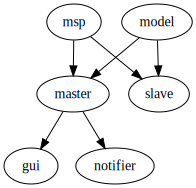
\includegraphics[height=5cm]{assets/module_graph}
\caption{Module Dependency Graph}
\end{figure}

\begin{itemize}
  \item Since the Master API was fully specified in the design document, GUI and notifier could be implemented indepenently.

  \item MSP and Model are mostly static datastructures and a simple transport mechanism.
        It was assumed they could be implemented quickly.

  \item Master and slave do not depend on each other code-wise, hence implementation could be parallelized, too.
\end{itemize}

Given these assumptions, it was attempted to distribute the work fairly between the team members, assuming cleanly separated
responsibilities would increase speed \& motivation through independent \& parallel work.

\begin{figure}[h]
\centering
\begin{tabular}{l|l}
        Component & Name\\
        \hline
        msp       & Anton\\
        model     & Christian\\
        master    & Anton, Christian\\
        slave     & Bob\\
        gui       & Janis\\
        notifier  & Niklas, Janis\\
\end{tabular}
\caption{Original Distribution of Work}
\end{figure}

This plan played out as follows:

\begin{itemize}
\item Initial versions of MSP and Model were implemented in a few days.
\item The master with its \textit{repository pattern} (independent modules with central database) proved as difficult to implement, as
      explained in \ref{di}.
\item The GUI implementation was straight forward. In particular, the AngularJS framework turned out to be a pleasant choice.
\item The notifier implementation was equally straight forward.
\item The initial slave implementation was finished early.
\end{itemize}

Two weeks prior to the phase deadline, integration of the individual components began:

\begin{itemize}
\item GUI and notifier worked flawlessly with the master API. The fact that the originally defined API endpoints were not changed
                but only new ones added was beneficial (see \ref{di:opneeds}).
\item Model and MSP worked well, apart from the consequences of migrating to PostgreSQL late in the implementation phase
        (see \ref{di:dbchanges}).
\item Integration of master and slave revealed flaws in the assumptions made about MongoDB in the design phase:
        \begin{itemize}
                \item a lot of unexpected Mongod behavior as described in \ref{di:replsetconfig} was only discovered at the
                        time of integration and required time-consuming test setups and debugging sessions.
                \item the addition of the keyfile requirement consumed a significant amount of time (3 days) in the
                       last seven days of the implementation phase (see \ref{di:keyfiles})
        \end{itemize}
\end{itemize}

The main conclusion drawn from this integration subphase is that master and slave should have been tested together earlier, allowing for
discovery and possibly more elegant handling of unexpected MongoDB behavior, as described in section \ref{di}.

\section{Testing}

\subsection{Unit Tests}

TODO elaborate on purpose of various unit tests.
possibly list all of them and elaborate on some in detail

\subsection{Integration Tets}

TODO explain why we have almost none and what we could do
, e.g. scripted API tests

\subsection{Manual Tests}


\section{Appendix}

In addition to this document, several manuals \& guides have been created during the implementation phase:

\begin{description}
\item[Updated Design Document] in the \codeinline{doc} repository.\\
      Represents the state of the implementation at the time of writing this document.
\item[README.md] in the \codeinline{code} repository.\\
      Gives guidance on setting up a developer machine for testing and building \mamid.
\item[INSTALL.md] in the \codeinline{code} repository.\\
      Gives guidance on deploying MAMID to a cluster, including 
      \begin{itemize}
        \item description of networking configuration
        \item help on how to use the bundled Certificate Authority helper scripts
        \item configuration for both testing and production setups
      \end{itemize}
\item[TESTING.md] in the \codeinline{code} repository.\\
      Gives guidance on how to setup the local staging environment mentioned in section \ref{dev:staging}.
\item[User Manual] for the GUI, accessible through the \mamid Web Interface (\textit{Help} button in the top bar)
\end{description}


\glsaddallunused
\makeatletter
\newglossarystyle{myAltlist}{
  \glossarystyle{altlist} % base this style on altlist
  \renewcommand*{\glossaryentryfield}[5]{
  \item[\glsentryitem{##1}\glstarget{##1}{##2}]
    \mbox{}\par\nobreak\@afterheading
    ##3\glspostdescription\space On page ##5.
  }
}
\makeatother

\end{document}
